\documentclass[../../main.tex]{subfiles}
\graphicspath{{../../image/}{../../figure/}}
\begin{document}

\section{构造格式}\label{section:ch13-构造格式}

我们考虑严格双曲守恒律系统的初值问题，定义在以原点为中心的球 $\mathcal{O}$ 上：
\begin{align}
\partial_t U(x,t)+\partial_x F(U(x,t))=0,\quad&-\infty<x<\infty,\ 0\leqslant t<\infty,\nonumber\\
U(x,0)=U_0(x),\quad&-\infty<x<\infty.
\label{align:ch13-ivp}
\end{align}
初始数据 $U_0$ 是 $(-\infty,\infty)$ 上的有界变差函数。最终目标是建立下述

\begin{theorem}[小总变差存在性]\label{theorem:ch13-小总变差存在性}
存在正常数 $\delta_0$ 与 $\delta_1$，使得当
\begin{align}
\sup_{(-\infty,\infty)}|U_0(\cdot)|<\delta_0,\label{align:ch13-sup-small}\\
TV_{(-\infty,\infty)}U_0(\cdot)<\delta_1,\label{align:ch13-tv-small}
\end{align}
时，存在\eqref{align:ch13-ivp}的一个解 $U$，它是 $(-\infty,\infty)\times[0,\infty)$ 上局部有界变差的函数，取值于 $\mathcal{O}$。该解对系统的任意熵--熵流对 $(\eta,q)$（其中 $\eta(U)$ 为凸）满足熵可容性准则。进而，对每个固定的 $t\in[0,\infty)$，$U(\cdot,t)$ 是 $(-\infty,\infty)$ 上的有界变差函数，并且
\begin{align}
\sup_{(-\infty,\infty)}|U(\cdot,t)|&\leqslant c_0\sup_{(-\infty,\infty)}|U_0(\cdot)|,\qquad 0\leqslant t<\infty,\label{align:ch13-sup-bound}\\
TV_{(-\infty,\infty)}U(\cdot,t)&\leqslant c_1TV_{(-\infty,\infty)}U_0(\cdot),\qquad 0\leqslant t<\infty,\label{align:ch13-tv-bound}\\
\int_{-\infty}^{\infty}|U(x,t)-U(x,\tau)|\,\mathrm{d}x&\leqslant c_2|t-\tau|\,TV_{(-\infty,\infty)}U_0(\cdot),\qquad 0\leqslant\tau<t<\infty,\label{align:ch13-lip-bound}
\end{align}
其中 $c_0,c_1,c_2$ 是仅依赖于 $F$ 的常数。当系统配备 Riemann 不变量坐标系时，\eqref{align:ch13-tv-small} 中的 $\delta_1$ 可任意大，只要
\begin{align}
\left(\sup_{(-\infty,\infty)}|U_0(\cdot)|\right)\left(TV_{(-\infty,\infty)}U_0(\cdot)\right)<\delta_2,
\label{align:ch13-product-small}
\end{align}
其中 $\delta_2$ 充分小，且依赖于 $\delta_1$。
\end{theorem}

上述命题的证明相当冗长，将占用整个章节。尽管结论在上述一般性层面上成立，但证明中的某些步骤（\cref{section:ch13-真非线性波相互作用}、\cref{section:ch13-glimm泛函}、\cref{section:ch13-总变差界}与\cref{section:ch13-上确界界}）将在简化假设下进行，即系统的每个特征族要么真非线性，要么线性退化。
一般系统的情形将在\cref{section:ch13-一般系统}与\cref{section:ch13-波追踪}中扼要提及。

解 $U$ 将作为一族近似解 $U_h$ 当 $h\downarrow0$ 时的极限而得到，该族近似解由下述过程构造。

固定空间步长 $h$（它将充当参数）以及相应的时间步长 $\lambda^{-1}h$，其中 $\lambda$ 是特征速度 $|\lambda_i(U)|$（$U\in\mathcal{O}$，$i=1,\cdots,n$）的固定上界。令 $x_r=rh$，$r=0,\pm1,\pm2,\cdots$，$t_s=s\lambda^{-1}h$，$s=0,1,2,\cdots$，我们构造网格点 $(x_r,t_s)$ 的交错网格，其中 $s=0,1,2,\cdots$，$r+s$ 为偶数。

现假设 $U_h$ 已在 $\{(x,t):-\infty<x<\infty,\ 0\leqslant t<t_s\}$ 上定义，我们把 $U_h(\cdot,t_s)$ 确定为一个阶梯函数，它在直线 $t=t_s$ 上由相邻网格点界定的区间上取常值：
\begin{align}
U_h(x,t_s)=U_s^r,\qquad x_{r-1}<x<x_{r+1},\ r+s\ \text{为奇数},
\label{align:ch13-step}
\end{align}
并逼近函数 $U_h(\cdot,t_s-)$。审慎选择常状态 $U_s^r$ 这一主要问题将在\cref{section:ch13-紧性与相容性}中处理。

接着我们把 $U_h$ 在带形 $\{(x,t):-\infty<x<\infty,\ t_s\leqslant t<t_{s+1}\}$ 上确定为系统的解，即
\begin{align}
\partial_t U_h(x,t)+\partial_x F(U_h(x,t))=0,\quad-\infty<x<\infty,\ t_s\leqslant t<t_{s+1},
\label{align:ch13-strip}
\end{align}
其中初始条件为直线 $t=t_s$ 上的\eqref{align:ch13-step}。注意，\eqref{align:ch13-strip}、\eqref{align:ch13-step}的解由从位于 $t_s$ 时间线上的网格点发出的中心波扇组成（见\cref{figure:ch13-交错网格}）。以网格点 $(x_r,t_s)$（$r+s$ 为偶数）为中心的波扇，通过求解系统的 Riemann 问题来构造，其左状态为 $U_s^{r-1}$、右状态为 $U_s^{r+1}$。我们采用可容许解，其中激波满足黏性激波可容性条件（参见第九章）。
由于我们选取了空间步长与时间步长之比 $\lambda$，从相邻网格点发出的出射波在时间区间 $[t_s,t_{s+1})$ 上不会相互作用。

\begin{figure}[ht]
\centering
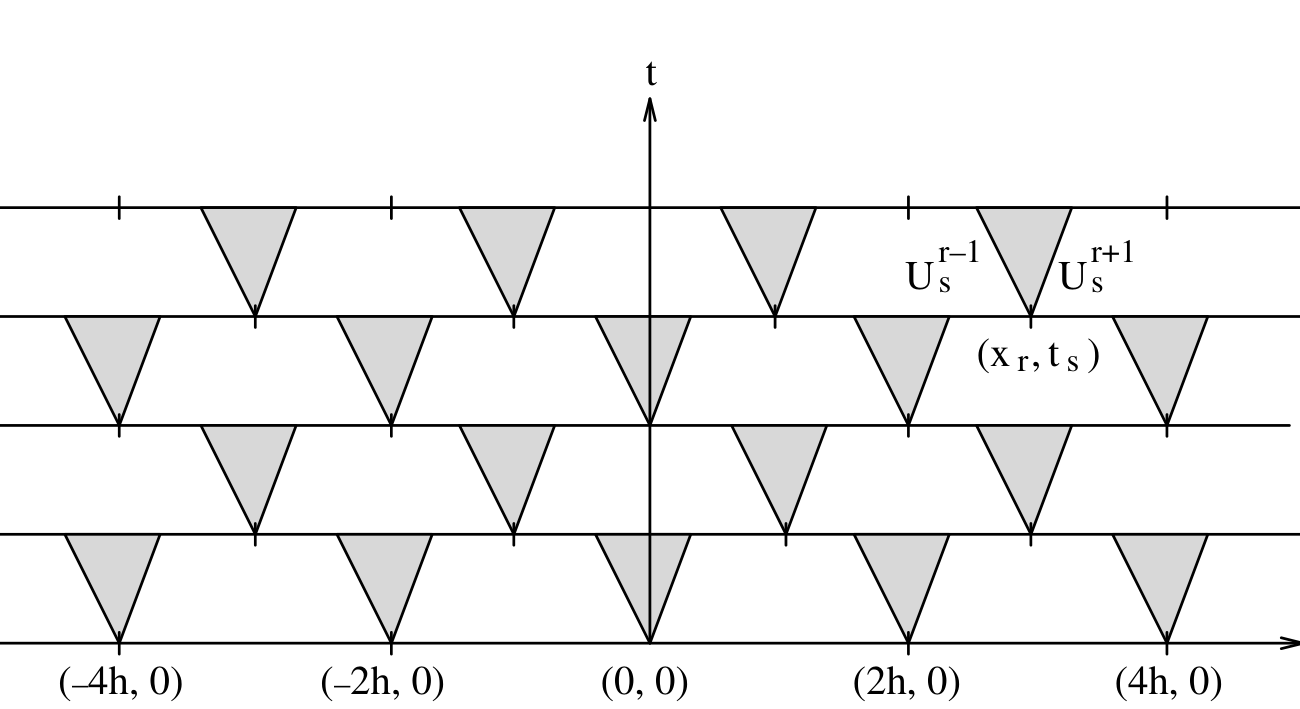
\includegraphics[width=0.85\textwidth]{ch13-fig01-01.png}
\caption{交错网格与中心波扇}\label{figure:ch13-交错网格}
\end{figure}

为启动算法，在 $s=0$ 时我们采用初始数据：
\begin{align}
U_h(x,0-)=U_0(x),\qquad-\infty<x<\infty.
\label{align:ch13-init}
\end{align}

只要能求解相应的 Riemann 问题，$U_h$ 的构造便可一直进行下去。正如在第九章中所见，这一般可在跳跃 $|U_s^{r+1}-U_s^{r-1}|$ 保持充分小时进行。

经过充分准备后，我们将在\cref{section:ch13-总变差界}与\cref{section:ch13-上确界界}中证明，$U_h$ 满足估计
\begin{align}
\sup_{(-\infty,\infty)}|U_h(\cdot,t)|&\leqslant c_0\sup_{(-\infty,\infty)}|U_0(\cdot)|,\qquad 0\leqslant t<\infty,\label{align:ch13-h-sup}\\
TV_{(-\infty,\infty)}U_h(\cdot,t)&\leqslant c_1TV_{(-\infty,\infty)}U_0(\cdot),\qquad 0\leqslant t<\infty,\label{align:ch13-h-tv}\\
\int_{-\infty}^{\infty}|U_h(x,t)-U_h(x,\tau)|\,\mathrm{d}x&\leqslant c_2(|t-\tau|+h)\,TV_{(-\infty,\infty)}U_0(\cdot),\qquad 0\leqslant\tau<t<\infty.
\label{align:ch13-h-lip}
\end{align}
特别地，当\eqref{align:ch13-sup-small}以充分小的 $\delta_0$ 成立时，\eqref{align:ch13-h-sup}保证 $U_h$ 可在整个上半平面上构造。

\end{document}